\documentclass[10pt]{article}

\usepackage{polski}
\usepackage{graphicx}
\usepackage{hyperref}
\usepackage{geometry}
\usepackage{fancyhdr}
\setlength{\headheight}{13.0pt}
\begin{document}

\graphicspath{{images/}}

\newgeometry{tmargin=4cm, bmargin=4cm, lmargin=3.2cm, rmargin=3.2cm} 

\pagestyle{fancy}

% Szablon przygotowany przez Jarosława Drapałę z dalszymi zmianami Michała Karola

\begin{titlepage}
\begin{center}
  
  \LARGE \textsc{Politechnika Wrocławska}\\
  \vspace*{0.2cm}
  \Large \textsc{Wydział Informatyki i Telekomunikacji}\\  
  \vspace*{0.4cm}
  \centering
\includegraphics[width=0.2\textwidth]{WITlogo.png}\\
  \vspace*{0.2cm}
  \vspace*{2cm}
        
  \centerline{\rule{\textwidth}{1.2pt}}
  \vspace{0.4cm}
  \Huge\textbf{Ocena win na podstawie danych aplikacji Vivino}
  \centerline{\rule{\textwidth}{1.2pt}}
  \vspace{1cm}
  \LARGE Sprawozdanie z laboratorium\\
  \vspace{3.5cm}
  \textsc{Autor}\\
  \vspace{0.2cm}
  \textbf{Inię Nazwisko}\\
  \vspace{0.1cm}
  \Large nr albumu: \textbf{123456}\\
  \vspace{0.1cm}
  kierunek: \textbf{Informatyka}
            
            
        
        
  \vspace*{\fill}
  \Large \textit{14 styczeń 2022}
            
 \end{center}


\end{titlepage}

\section{Wstęp -- sformułowanie problemu}
\label{sec:wstep}

Autor porzebuje określić najoptymalniejsze miejsca na wybudowanie nowego parku w mieście San Francisco na podstawie istniejących już parków oraz szkół.\\
Rozwiąznie tego problemu pozwoli na podniesienie poziomu życia oraz zadowolenia mieszkańców w mieście.

\section{Opis danych}
Do rozwiązania problemu będą wykorzystywane 2 datasety.\\\\
Pierwszym z nich jest lokalizacja wszystkich instniejących parków - rozmiar 240 wierszy. \\
Kolumna "shape" - określa kształ parku, który zostaje zamienony na punkt - środek parku reprezentujący jego położenie.\\ \\
Drugim z nich jest położenie wszystkich szkół - rozmiar 445 wierszy.\\
Kolumna "location\_1" - zmienna określająca długość oraz szerokośc geograficzną obiektu, reprezentuje punkt na mapie.

\section{Opis rozwiązania}

Dane zostały pobrane ze strony \url{https://data.sfgov.org/}. Dostęp do danych uzyskano za pomocą API, natomiast w przypadku wykorzystywanych datasetów nie był potrzebny do tego klucz prywatny, ponieważ są to dane dostępne publicznie. Baza została zapisana w postaci ramki danych korzystacjąc z biblioteki \texttt{Pandas}, a następnie przetworzone tak, aby każdy obiekt był reprezentowany przez dwie wartości - \texttt{x, y}. Tak przygotowane dane zostały następnie przetworzone przy wykorzystaniu biblioteki \texttt{constraint}, która pozwala na określenie ograniczeń oraz danych, którymi w naszym przypadku są położenia szkół oraz istniejących już parków. Dzięki temu uzyskamy model reprezentujący najbardziej optymalne miejsca budowy.

\section{Rezultaty obliczeń}

\subsection{Plan badań}
Do przeprowadzenia badań musimy określić ograniczenia, którymi algorytm będzie się kierował. W tym przypadku dobór wartości jest następujący:
\begin{enumerate}
    \item Minimalna i maksymalna odległość od istniejącej szkoły: ~0.95km, ~1km
    \item Minimalna i maksymalna odległośc od istniejącego parku: ~4km, ~4.2km
    \item Przedział przeszukiwanych położeń dla x: minimalna oraz maksymalna wartość długości geograficznej istniejących parków.
    \item Przedział przeszukiwanych położeń dla y: minimalna oraz maksymalna wartość szerokości geograficznej istniejących parków.
\end{enumerate}

Tak dobrane wartości pozwalają na stworzenie formuł reprezentujących nasze ograniczenia.\\
Położenia spełniające warunek odległości od istniejącej szkoły:
\[ distance = (new\_pos\_x - school\_x)^2 + (new\_pos\_y - school\_y)^2 \]
\[if distance > min\_school\_distance^2 and distance < max\_school\_distance^2: True\]
Następnie ze znalezionych pozycji możemy wybrać te, które spełniają warunek odległości od istniejącego parku:
\[distance = (found\_position\_x - park\_x)^2 + (found\_position\_y - park\_y)^2\]
\[if distance > min\_park\_distance^2 and distance < max\_park\_distance^2: True\]

Gdzie distance w obu przypadkach oznacza odległość punktu od danego obiektu, new\_pos oznacza nową pozycję, która będzie sprawdzana, a school\_x, school\_y, park\_x, park\_y oznaczają kolejno położenia aktualnie sprawdzanych szkół i parków.\\
Dla optymalizacji programu wykorzystano podniesie zmiennych reprezentujących maksymalny i minimalny dystans od danego obiektu do kwadratu, tak aby uniknąć pierwiastkowania przy obliczaniu odległości między dwoma punktami.
\newpage
\subsection{Wyniki obliczeń}
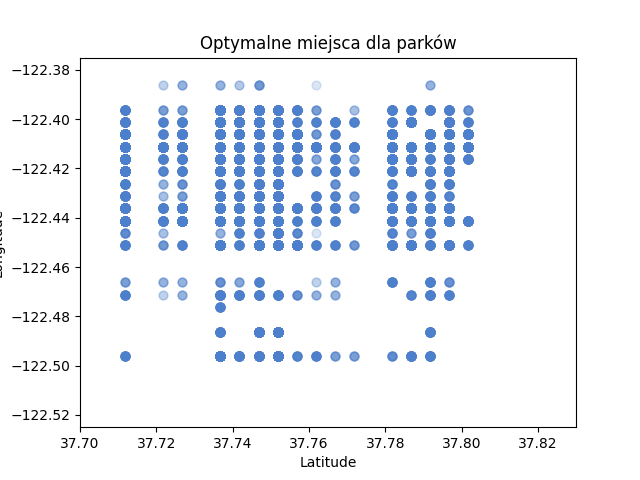
\includegraphics[width = 15cm]{images/plots/optimal_parks.png}
\newline 
Otrzymane wyniki można zaprezentować na wykresie, reprezentującym długość oraz szerokość geograficzną jako punkty.
\section{Wnioski}
Przedstawiona metoda pozwala na wyszukiwanie optymalnych miejsc na podstawie informacji o istniejących obiektach. Warto zauważyć, że przy pobieraniu datasetu należy zwrócić uwagę na rozłożenie zmiennych określających długość i szerokość geograficzną, jako iż mogą one występować zamiennie.\\
Należy również podkreślić, że w celach wykonania projektu, dataset został zmniejszony odpowiednio do rozmiaru 100 wierszy, tak aby algorytm wykonał się w realnym czasie.\\
Jak widzimy na załączonym wykresie, otrzymaliśmy zbiór najbardziej optymalnych miejsc na wybudowanie nowego parku, reprezentowanych jako punkty. Takie informacje można wykorzystać w procesie planowania kolejnych inwestycji, tak aby stosunek kosztów do wartości publicznej był jak największy.

\appendix
\section{Dodatek}
Kody źródłowe(utrzymane w konwencji języka Python wraz z instrukcjmi uruchomienia) umieszczone zostały w repozytorium github:

\noindent \url{github.com/Jakub-Bednarek/MSiD-Project}.


\end{document}